% ============================================================================
% TWO-STAGE RANDOMIZED TRIAL DESIGN FOR ANTIMICROBIALS: EPIDEMIOLOGY VERSION
% Formatted for Epidemiology (Lippincott Williams & Wilkins)
% ============================================================================

\documentclass[12pt]{article}

\usepackage[margin=1in]{geometry}
\usepackage{amsmath}
\usepackage{amssymb}
\usepackage{tikz}
\usepackage{booktabs}
\usepackage{graphicx}
\usepackage{multirow}
\usepackage{setspace}
\usepackage[super,comma,sort&compress]{natbib}
\usepackage{caption}
\usepackage{array}
\usetikzlibrary{shapes,arrows,arrows.meta,calc,positioning}

% Epidemiology uses superscript numbered references
\renewcommand{\bibnumfmt}[1]{#1.}


\begin{document}

% --- Title Page ---
\begin{titlepage}
\centering
{\Large Original Research Article}\\[2em]
{\LARGE\bfseries Advantages of a Two-Stage Randomized Trial Design to Evaluate Antimicrobial Treatment Strategies: a Simulation Study}\\[2em]

\textbf{Juan Gago}$^{1}$\textsuperscript{*}, \textbf{Christopher Boyer}$^{1,2,3}$, \textbf{Marc Lipsitch}$^{1}$\\[1em]

{\small
$^1$ Department of Epidemiology, Harvard T.H. Chan School of Public Health, Boston, MA, USA\\
$^2$ Department of Medicine, Case Western Reserve School of Medicine, Cleveland, OH, USA\\
$^3$ Department of Quantitative Health Sciences, Cleveland Clinic, Cleveland, OH, USA\\[1em]
\textsuperscript{*}Corresponding author: Juan Gago, 677 Huntington Avenue, Kresge Building, Suite 506. Boston, MA 02115. Email: juangago@hsph.harvard.edu
}\\[2em]

\textbf{Running head:} Two-stage randomized design for antimicrobials\\[1em]
\textbf{Conflict of Interest:} The authors declare no conflicts of interest.\\[0.5em]
\textbf{Funding:} This work was supported by VK Fund for the CCDD.\\[0.5em]
\textbf{Keywords:} Causal inference, interference, drug resistance, antimicrobials, agent-based models, study design.\\[0.5em]
\textbf{Data and Code Availability:} Simulation code available upon request.\\[0.5em]

\end{titlepage}

\newpage

% --- Structured Abstract ---
\noindent\textbf{ABSTRACT}\\[0.5em]

\noindent\textbf{Background:} Antimicrobial prescribing policies affect not only treated patients but also others through altered transmission dynamics. Two-stage randomized (2SR) designs can estimate both direct and indirect effects, yet have not been applied to antimicrobial strategies.\\[0.3em]

\noindent\textbf{Methods:} We developed a stochastic agent-based model simulating a hospital ward with two competing bacterial strains (drug-susceptible and drug-resistant). We emulated a 2SR trial: 6 clusters were randomized to a 90/10 (90\% narrow-spectrum Drug~A) or 50/50 allocation strategy; individuals within clusters were then randomized to Drug~A or Drug~B (broad-spectrum). We estimated direct, indirect, total, and overall causal effects on all-cause mortality following Hudgens and Halloran. Sensitivity analyses varied the treatment effect, transmission rate, mortality structure, and number of clusters.\\[0.3em]

\noindent\textbf{Results:} Drug~A recipients had 2.80--4.60 percentage points (pp) higher mortality than Drug~B recipients (direct effect), attributable to non-concordant treatment of resistant infections. The indirect effect on Drug~A recipients was $+$1.75~pp, reflecting higher resistant-strain prevalence under 90/10. The 50/50 strategy reduced total deaths (603 vs.\ 888) but paradoxically increased susceptible infections (9,625 vs.\ 7,599) through competitive exclusion. All findings were robust across sensitivity analyses.\\[0.3em]

\noindent\textbf{Conclusions:} Antimicrobial prescribing policies interact with transmission dynamics through strain competition. The 2SR design captures spillover effects that individually randomized trials cannot detect, providing a framework for future antimicrobial trials and observational emulations.\\[1em]

\clearpage
\doublespacing

\section*{Introduction}

Antimicrobial resistance (AMR) threatens to undermine gains of modern medicine by reducing treatment effectiveness.\cite{lipsitch_epidemiology_2000} The challenge for clinicians and policymakers is to identify antimicrobial strategies that achieve two goals simultaneously: treating infections effectively in the individual patient and limiting the emergence and spread of resistance in the population.

Most evidence on antimicrobial therapies comes from individually randomized trials. These trials estimate the causal effect of treatment on treated patients but provide little information about spillover effects---how the treatment of one patient may affect the outcomes of others through transmission of susceptible and resistant organisms. Ignoring these indirect effects is problematic because antimicrobial use in one individual can alter the risk faced by others.\cite{gago_how_2025}

Two-stage randomized (2SR) designs provide a framework for simultaneously estimating direct and indirect effects.\cite{hudgens_toward_2008} Clusters (e.g., hospital wards) are first randomized to different levels of treatment coverage, and then individuals within clusters are randomized to treatment strategies consistent with the cluster assignment. Such designs have been applied to vaccines and HIV prevention interventions, where indirect effects are expected to be substantial,\cite{buchanan_disseminated_2021} and recent work has formalized their connection to the target trial framework.\cite{murray_emulating_2021} To our knowledge, no applications have been developed for antimicrobial treatment strategies, despite the centrality of indirect effects to AMR dynamics.

Other approaches have addressed population-level AMR. Observational studies and mechanistic models suggest antimicrobial use influences resistance prevalence at the population level,\cite{pham_characterizing_2025,olesen_role_2020} but face well-known threats to causal identification. A few cluster-randomized antimicrobial trials exist. Van Duijn et al.\cite{duijn_effects_2018} conducted a cluster-randomized crossover trial of antibiotic cycling versus mixing across European ICUs, but the design compared two ward-level policies without individual-level randomization, precluding separation of direct and indirect effects. Arzika et al.\cite{arzika_spillover_2025} analyzed spillover in the AVENIR trial of mass azithromycin distribution in Niger, finding that treating older siblings (children 1--59 months) reduced infant mortality beyond direct protection---the first antimicrobial trial to formally estimate spillover on survival. However, that design randomized communities to coverage levels without individual-level randomization within communities, so direct and indirect effects could not be disentangled. Neither trial adopted the two-stage structure needed to simultaneously identify both components. Agent-based models (ABMs) have explored related questions, such as the evaluation of carbapenem-resistant \textit{Enterobacterales} decolonization strategies,\cite{toth_economic_2021} but they have not been structured to emulate 2SR designs for antimicrobials.

In this paper, we extend the 2SR framework to antimicrobial strategies by implementing it in an ABM. We define clusters as hospital wards and randomize both cluster-level coverage (the proportion of patients treated with broad-spectrum Drug~B) and individual-level treatment assignment (which specific drug a patient receives). The ABM serves as the data-generating mechanism from which the target 2SR trial is emulated, allowing us to quantify direct, indirect, and overall effects of antimicrobial prescribing policies under controlled conditions.

\section*{Methods}

\subsection*{Model Setup}

We developed a discrete-time, stochastic ABM to simulate a 2SR trial of antimicrobial treatment strategies in a hospital setting. Each agent represents an individual patient followed over 350 timesteps within a simulated ward structure. We used R software version 4.4.1 and the ABM package (version 0.4.3) for simulations.

Each agent occupies one of the following mutually exclusive health states: uninfected ($X$); colonized with a drug-susceptible ($S$) or drug-resistant ($R$) strain; symptomatic and treated with Drug~A or Drug~B ($TS_A$, $TS_B$, $TR_A$, $TR_B$); symptomatic and untreated ($US$, $UR$); discharged alive ($Z$); or deceased ($D$). The state-transition diagram is provided in eFigure~1.

\subsubsection*{Admission and Discharge.}
Admissions follow a Poisson process at rate $\lambda = 10$. New admissions enter state $X$ (uninfected) with probability $m = 0.75$, or state $S$ (susceptible infection) with probability $1 - m$. No new admissions arrive with resistant infections; all resistance in the model arises from within-ward transmission. Discharge ($Z$) and death ($D$) transitions apply only to symptomatic or treated agents, at rates $\mu = 0.095$ and $\delta = 0.025$ (with state-specific multipliers), respectively.

\subsubsection*{Transmission.}
Homogeneous mixing within wards leads to:
\[
  X + S \xrightarrow{\beta} S + S, \qquad
  X + R \xrightarrow{\beta(1 - c)} R + R,
\]
where $\beta = 0.4$ is the transmission rate and $c = 0.02$ is the fitness cost of resistance.

\subsubsection*{Symptom Onset and Treatment.}
Symptom onset occurs at rate $\sigma = 1$ (rapid onset, effectively collapsing the latent period). Symptomatic agents enter treatment with probability $\rho = 0.9$, receiving Drug~A with cluster-specific probability $\pi$ and Drug~B with probability $1 - \pi$. Untreated symptomatic patients remain in $US$ or $UR$.

\subsubsection*{Recovery.}
Recovery transitions are:
\[
  TS_A,\, TS_B \xrightarrow{\gamma + \tau} X, \quad
  US \xrightarrow{\gamma} X, \quad
  TR_B \xrightarrow{\gamma + \tau} X, \quad
  TR_A,\, UR \xrightarrow{\gamma} X,
\]
with $\gamma = 0.20$ and treatment effect $\tau = 0.7$. The treatment effect accelerates recovery for concordant therapy: both drugs cover susceptible infections, but only Drug~B covers resistant infections. Drug~A recipients with resistant infections ($TR_A$) recover at the untreated rate.

\subsubsection*{Mortality Rates by Stratum.}
The primary outcome is all-cause mortality. The baseline death rate $\delta = 0.025$ is modified by state-specific multipliers: treated susceptible ($TS_A$, $TS_B$) and concordant resistant ($TR_B$): $1\times\delta$; untreated susceptible ($US$): $1.5\times\delta$; non-concordant resistant ($TR_A$): $2\times\delta$; and untreated resistant ($UR$): $3\times\delta$. These reflect the assumption that untreated infections carry higher mortality, and that resistant infections treated with a non-concordant drug have elevated mortality.

\begin{table}[htbp]
\centering
\caption{Model parameters.}
\label{tab:parameters}
{\small
\begin{tabular}{llll}
\toprule
\textbf{Parameter} & \textbf{Symbol} & \textbf{Value} & \textbf{Justification} \\
\midrule
Admission rate & $\lambda$ & 10 & Maintains $\approx$1000 agents \\
Prob.\ uninfected admission & $m$ & 0.75 & Baseline prevalence \\
Initial S/R infected & $S_0$, $R_0$ & 50 & Seeds infection pressure \\
Transmission rate & $\beta$ & 0.4 & Within-ward contact rate \\
Fitness cost of resistance & $c$ & 0.02 & Reduced R transmissibility \\
Recovery rate & $\gamma$ & 0.20 & Mean duration 5 timesteps \\
Treatment effect & $\tau$ & 0.7 & 78\% reduction in infectious period \\
Symptom onset rate & $\sigma$ & 1.0 & Rapid (collapsed latent period) \\
Treatment probability & $\rho$ & 0.9 & High uptake \\
Discharge rate & $\mu$ & 0.095 & Balances admissions \\
Baseline death rate & $\delta$ & 0.025 & 2.5\% baseline mortality \\
Prob.\ Drug~A ($\alpha_1$) & $\pi$ & 0.90 & 90/10 strategy \\
Prob.\ Drug~A ($\alpha_0$) & $\pi$ & 0.50 & 50/50 strategy \\
\bottomrule
\end{tabular}
}
\\[0.3em]
\footnotesize
\textit{Note:} Sensitivity analyses were performed on $\tau$, $\beta$, $\delta$, and number of clusters.
\end{table}

\subsubsection*{Simulation Procedure.}
We initialized 1,000 agents (50 in $S$, 50 in $R$, remainder in $X$) and simulated 6 clusters: 3 assigned to $\pi = 0.9$ (90/10 strategy, $\alpha_1$) and 3 to $\pi = 0.5$ (50/50 strategy, $\alpha_0$). Each cluster was replicated 10 times to capture stochastic variability, yielding 60 total simulation runs.

\subsection*{Causal Framework}

We define causal effects within the potential outcomes framework under the assumption of \textit{partial interference}\cite{hudgens_toward_2008,sobel_what_2006} and \textit{stratified interference}.\cite{hudgens_toward_2008} Let $\mathbf{z}_i = (z_{i1}, \ldots, z_{in_i})$ denote the treatment vector for cluster $i$, where $z_{ij} \in \{A, B\}$. The potential outcome for individual $j$ in cluster $i$ is $Y_{ij}(\mathbf{z}_i)$.

Under partial interference, an individual's outcome may depend on treatments assigned to others in their cluster, but not on treatments in other clusters:
\begin{equation}
Y_{ij}(\mathbf{z}_1, \ldots, \mathbf{z}_K) = Y_{ij}(\mathbf{z}_i).
\end{equation}
Under stratified interference, $Y_{ij}(\mathbf{z}_i)$ depends on $\mathbf{z}_i$ only through (a) the individual's own treatment $z_{ij}$ and (b) the allocation strategy $\alpha(\mathbf{z}_i)$. These assumptions relax the standard Stable Unit Treatment Value Assumption (SUTVA) and enable us to define individual average potential outcomes $\bar{Y}_{ij}(a, \alpha)$.

Let $\bar{Y}(a, \alpha)$ denote the population-average potential outcome under treatment $a \in \{A, B\}$ and strategy $\alpha$, and $\bar{Y}(\alpha)$ the marginal average under $\alpha$. Following Hudgens and Halloran,\cite{hudgens_toward_2008} we define:
\begin{align}
\mathrm{DE}(\alpha_0) &= \bar{Y}(A, \alpha_0) - \bar{Y}(B, \alpha_0), \label{eq:de0}\\
\mathrm{DE}(\alpha_1) &= \bar{Y}(A, \alpha_1) - \bar{Y}(B, \alpha_1), \label{eq:de1}\\
\mathrm{IE}(A) &= \bar{Y}(A, \alpha_1) - \bar{Y}(A, \alpha_0), \label{eq:iea}\\
\mathrm{IE}(B) &= \bar{Y}(B, \alpha_1) - \bar{Y}(B, \alpha_0), \label{eq:ieb}\\
\mathrm{TE} &= \bar{Y}(A, \alpha_1) - \bar{Y}(B, \alpha_0), \label{eq:te}\\
\mathrm{OE} &= \bar{Y}(\alpha_0) - \bar{Y}(\alpha_1), \label{eq:oe}
\end{align}
where $\alpha_0$ denotes the 50/50 strategy and $\alpha_1$ denotes the 90/10 strategy. DE is the direct effect (own treatment, holding strategy fixed), IE the indirect (spillover) effect (strategy, holding treatment fixed), TE the total effect, and OE the overall (policy-level) effect. Positive values indicate higher mortality; negative OE indicates that the 50/50 strategy reduces mortality. The TE decomposes as $\mathrm{DE}(\alpha_1) + \mathrm{IE}(B)$ or equivalently $\mathrm{IE}(A) + \mathrm{DE}(\alpha_0)$.

Because both cluster-level strategy and individual treatment are randomized, exchangeability, consistency, and positivity hold by design. When emulating this design with observational data, confounding adjustment at both levels would be essential.\cite{tchetgen_tchetgen_causal_2012}

\subsubsection*{Inference and Simulation Intervals.}
Point estimates were computed by averaging outcomes across replicates. Ninety-five percent simulation intervals (SI) were computed as empirical 2.5th--97.5th percentiles across 10 replicates per cluster-strategy combination. SIs reflect Monte Carlo variability but do not quantify uncertainty from model misspecification.

\textit{Note on sign convention:} All estimands are defined such that positive values indicate higher mortality in the first term. The OE is defined as $\alpha_0$ minus $\alpha_1$, so a negative OE indicates that the 50/50 strategy reduces mortality.

\subsection*{Sensitivity Analyses}

We conducted one-way sensitivity analyses varying four dimensions independently: (1) mortality structure (uniform $\delta = 0.025$ across all states); (2) treatment effect magnitude ($\tau \in \{0.3, 0.7, 1.0\}$); (3) transmission rate ($\beta \in \{0.2, 0.4, 0.6\}$); and (4) cluster configuration (3 vs.\ 6 clusters per arm).

\section*{Results}

The simulation comprised 6 hospital wards, with 3 randomized to the 90/10 strategy and 3 to the 50/50 strategy. Each ward was initialized with 1,000 agents, with mean admissions of 10 per timestep and discharge and death rates approximately balancing the admission flow. Under the 50/50 strategy, resistant strains were suppressed while susceptible infections dominated; under the 90/10 strategy, resistant strains persisted at higher prevalence.

\subsection*{Causal Effects}

Table~\ref{tab:estimands} presents the causal effect estimates. The direct effect of Drug~A versus Drug~B was positive under both strategies (DE($\alpha_0$) = $+2.80$~percentage points [pp]; DE($\alpha_1$) = $+4.60$~pp), indicating higher mortality among Drug~A recipients. This is expected: Drug~A does not cover resistant infections, so patients with resistant infections treated with Drug~A face the elevated $TR_A$ mortality rate ($2\delta = 0.05$), while Drug~B covers both strain types. The direct effect is larger under the 90/10 strategy, where greater Drug~A use means a larger fraction of resistant-infected patients receive non-concordant therapy.

For Drug~B recipients, the indirect effect was approximately null (IE(B) = $-0.05$~pp; 95\% SI: $-0.90$, $+0.46$), suggesting minimal spillover on B-treated patients' mortality. For Drug~A recipients, the indirect effect was positive and larger (IE(A) = $+1.75$~pp; 95\% SI: $+0.72$, $+3.49$), reflecting that under the 90/10 strategy, A-treated patients face a ward environment with substantially higher resistant-strain prevalence; since Drug~A does not cover resistant infections, this shifts the case mix toward non-concordant treatment, raising mortality. These patterns are visible in Figure~\ref{fig:cumulative_deaths}, where panel~A shows the 90/10 strategy producing substantially more resistant-strain deaths, while panel~B reveals that even susceptible-strain deaths diverge between strategies, reflecting indirect effects operating through altered transmission dynamics.

The overall effect was $-2.68$~pp (95\% SI: $-3.90$, $-1.96$): the 50/50 strategy yielded 603 total deaths versus 888 under 90/10 (Table~\ref{tab:outcomes}), a reduction of 285 deaths. However, this benefit was distributed unevenly by infection type. Resistant-infected patients benefited substantially from greater Drug~B availability (fewer deaths: 266 vs.\ 628). Conversely, susceptible-infected patients experienced modestly higher mortality under 50/50 (337 vs.\ 260 deaths), driven by higher cumulative incidence of susceptible infections when resistant strains are suppressed (Figure~\ref{fig:cumulative_incidence}, Table~\ref{tab:risk_summary}).

\begin{table}[htbp]
\centering
\caption{Causal effect estimates (percentage points) with 95\% simulation intervals. $\alpha_0$ = 50/50 strategy; $\alpha_1$ = 90/10 strategy.}
\label{tab:estimands}
{\small
\begin{tabular}{lcccc}
\toprule
\textbf{Estimand} & \textbf{Definition} & \textbf{Estimate} & \textbf{95\% SI} & \textbf{Interpretation} \\
\midrule
\multicolumn{5}{l}{\textit{A. Direct Effects (Drug A vs B within each strategy)}} \\
DE($\alpha_0$) & $\bar{Y}(A, \alpha_0) - \bar{Y}(B, \alpha_0)$ & $+2.80$ & [$+1.78$, $+3.45$] & Own-treatment effect at 50/50 \\
DE($\alpha_1$) & $\bar{Y}(A, \alpha_1) - \bar{Y}(B, \alpha_1)$ & $+4.60$ & [$+3.80$, $+5.61$] & Own-treatment effect at 90/10 \\
\midrule
\multicolumn{5}{l}{\textit{B. Indirect Effects (90/10 vs 50/50 within each drug)}} \\
IE(A) & $\bar{Y}(A, \alpha_1) - \bar{Y}(A, \alpha_0)$ & $+1.75$ & [$+0.72$, $+3.49$] & Spillover on A-treated \\
IE(B) & $\bar{Y}(B, \alpha_1) - \bar{Y}(B, \alpha_0)$ & $-0.05$ & [$-0.90$, $+0.46$] & Spillover on B-treated \\
\midrule
\multicolumn{5}{l}{\textit{C. Total and Overall Effects}} \\
TE & $\bar{Y}(A, \alpha_1) - \bar{Y}(B, \alpha_0)$ & $+4.56$ & [$+4.09$, $+5.41$] & DE($\alpha_1$) $+$ IE(B) \\
OE & $\bar{Y}(\alpha_0) - \bar{Y}(\alpha_1)$ & $-2.68$ & [$-3.90$, $-1.96$] & Policy-level effect \\
\bottomrule
\end{tabular}
}
\\[0.3em]
\footnotesize
\textit{Note:} Positive values = higher mortality in the first term. OE negative = 50/50 reduces mortality. SIs are empirical 2.5th--97.5th percentiles across 10 replicates.
\end{table}

\begin{figure}[htbp]
  \centering
  
\includegraphics[width=\textwidth]{fig3_cumulative_deaths.png}
  \caption{Cumulative deaths by allocation strategy. (A) Deaths from resistant infections: the 90/10 strategy produces substantially more resistant-strain deaths. (B) Deaths from susceptible infections: the 50/50 strategy produces modestly more susceptible-strain deaths, reflecting competitive exclusion. (C) Total deaths: the 50/50 strategy yields lower overall mortality. Faint lines show individual simulation runs; bold lines show means across 10 replicates; ribbons indicate $\pm$1~SE.}
  \label{fig:cumulative_deaths}
\end{figure}

\subsection*{Infection and Mortality Outcomes}

Table~\ref{tab:outcomes} summarizes key outcomes by allocation strategy and infection type. The 50/50 strategy led to lower cumulative resistant infections (2,560 vs.\ 4,283) and fewer resistant-related deaths (266 vs.\ 628). Conversely, susceptible infection incidence was higher (9,625 vs.\ 7,599) and so was susceptible-related mortality (337 vs.\ 260). This trade-off is the hallmark of the spillover effect: Drug~B--intensive therapy reduces resistance at the cost of increased susceptible-strain transmission (Figure~\ref{fig:cumulative_incidence}). This trade-off would be invisible to a standard individually randomized trial.

\begin{table}[htbp]
\centering
\caption{Cumulative infection incidence and deaths by allocation strategy.}
\label{tab:outcomes}
{\small
\begin{tabular}{lcccc}
\toprule
\textbf{Strategy} & \textbf{Cumul.\ S Infec.} & \textbf{Cumul.\ R Infec.} & \textbf{Deaths (S)} & \textbf{Deaths (R)} \\
\midrule
50/50 & 9,625 & 2,560 & 337 & 266 \\
90/10 & 7,599 & 4,283 & 260 & 628 \\
\bottomrule
\end{tabular}
}
\end{table}

\begin{figure}[htbp]
  \centering
  
\includegraphics[width=\textwidth]{fig4_cumulative_incidence.png}
  \caption{Cumulative new infections by allocation strategy and infection type. Under the 50/50 strategy, susceptible infections accumulate substantially more than under 90/10, while resistant infections are suppressed. This reversal illustrates the competitive exclusion mechanism: suppressing resistant strains with Drug~B releases susceptible strains from ecological competition.}
  \label{fig:cumulative_incidence}
\end{figure}

\begin{table}[htbp]
\centering
\caption{Risk of death by infection type and allocation strategy, with risk differences (RD).}
\label{tab:risk_summary}
{\small
\begin{tabular}{lcccccc}
\toprule
& \multicolumn{2}{c}{Susceptible} & \multicolumn{2}{c}{Resistant} &
\multirow{2}{*}{RD} & \multirow{2}{*}{95\% SI} \\
\cmidrule(lr){2-3} \cmidrule(lr){4-5}
Strategy & Risk & SE & Risk & SE &  &  \\
\midrule
50/50 & 0.0350 & 0.0006 & 0.1030 & 0.0023 &  &  \\
90/10 & 0.0342 & 0.0006 & 0.1470 & 0.0017 &  &  \\
\midrule
RD Susceptible &  &  &  &  & $-$0.0008 & [$-$0.006, $+$0.003] \\
RD Resistant &  &  &  &  & $+$0.044 & [$+$0.035, $+$0.059] \\
\bottomrule
\end{tabular}
}
\end{table}

\subsection*{Mechanism: Competitive Exclusion}

The biological mechanism driving the spillover effect is competitive exclusion between strains. When Drug~B use is low (90/10 strategy), resistant strains are less suppressed and maintain higher prevalence, reducing the ecological niche available for susceptible-strain transmission. Conversely, when Drug~B use is high (50/50 strategy), resistant prevalence is suppressed, allowing susceptible strains to exploit the freed transmission space. The net effect on mortality is complex: while the 50/50 strategy prevents resistant-strain deaths, it paradoxically increases susceptible-strain incidence, which also causes mortality. Stewardship policies thus interact with transmission dynamics in non-obvious ways---a phenomenon that the two-stage design is uniquely positioned to capture.

\subsection*{Sensitivity Analyses}

Under uniform mortality hazards ($\delta = 0.025$ for all states), spillover effects persisted in the same direction, confirming that indirect effects exist independently of differential outcome severity.

As $\tau$ increased from 0.3 to 1.0, IE(A) grew from $+0.96$~pp (SI: $+0.30$, $+1.81$) to $+2.71$~pp (SI: $+1.64$, $+3.80$), and OE strengthened from $-1.63$~pp to $-3.46$~pp. The qualitative pattern---50/50 reduces total mortality at the cost of increased susceptible infections---was preserved at all values of $\tau$, but effect magnitudes scaled with treatment efficacy.

At low transmission ($\beta = 0.2$), effects were attenuated (IE(A) = $+0.46$~pp; OE = $-0.73$~pp); at high transmission ($\beta = 0.6$), effects were amplified (IE(A) = $+1.70$~pp; OE = $-3.03$~pp), with wider SIs reflecting greater stochastic variability. The qualitative direction was preserved across all transmission rates.

With 6 clusters per arm (vs.\ 3 baseline), IE(A) = $+2.00$~pp (SI: $+1.41$, $+2.96$) and OE = $-2.88$~pp (SI: $-3.48$, $-2.64$). Effect estimates were stable with overlapping SIs, suggesting that 3 clusters per arm is sufficient for qualitative inference.

\section*{Discussion}

This simulation study demonstrates that a 2SR design is both feasible and informative for evaluating antimicrobial treatment strategies. The design estimated direct effects of drug choice (Drug~A recipients had 2.80--4.60~pp higher mortality), indirect effects via altered population transmission (spillover effects on same-drug recipients across strategies), and overall effects (population-level mortality reduction under Drug~B--intensive strategies). The spillover effect---the paradoxical increase in susceptible infections under the 50/50 strategy, driven by competitive exclusion---would be completely undetectable in a standard individually randomized trial.

The competitive exclusion mechanism has important implications for stewardship. When broad-spectrum (Drug~B) use is high, resistant strains are suppressed and their prevalence falls. However, this releases susceptible strains from competition, leading to higher susceptible-strain incidence. While the 50/50 strategy prevents resistant-strain disease directly (fewer R-related deaths: 266 vs.\ 628), the population-level consequence is a redistribution of infections toward susceptible strains. Stewardship policies that focus narrowly on minimizing broad-spectrum use may inadvertently reshape strain ecology.\cite{lipsitch_epidemiology_2000,olesen_role_2020}

The 2SR design should be considered for future antimicrobial trials where: (1) indirect effects via transmission are expected to be substantial; (2) ecological dynamics may alter outcomes of interest; (3) spillover effects on untreated patients are a policy concern; and (4) the intervention operates at a system level (stewardship policies, prescribing guidelines). Our sensitivity analyses confirm that results are robust across a range of parameter values, though real trials would require more clusters for formal hypothesis testing.

The target trial framework, combined with ABM emulation, provides a roadmap for observational emulation. One would define clusters as hospital wards, identify prescribing strategies, control for confounders at both levels (ward type, patient acuity, baseline resistance), and estimate effects using inverse probability weighting or g-computation.\cite{tchetgen_tchetgen_causal_2012} Electronic health records from hospital networks could support such emulation. The stratified interference assumption requires that confounding be controlled within clusters; unmeasured cross-cluster effects would violate partial interference.

This study has several limitations. The model assumes homogeneous mixing and no cross-cluster transmission; real hospitals have heterogeneous contact networks. Only 6 clusters were simulated (3 per arm). The model omits de novo resistance emergence, patient heterogeneity, polymicrobial infections, and prior antibiotic exposure. Treatment allocation was deterministic; clinician behavior would be heterogeneous in reality. Despite these simplifications, the simulation demonstrates the principle that 2SR designs can detect spillover effects that conventional designs cannot, providing proof-of-concept for future applications.

This work establishes a framework for using 2SR designs and ABM emulation to evaluate antimicrobial strategies in the context of transmission dynamics and resistance. A practical next step would be to implement a 2SR stewardship trial in a hospital system to determine whether population-level prescribing changes achieve the intended goal of reducing resistance without shifting disease burden to other pathogens.

\section*{Acknowledgments}

The authors acknowledge support from the VK Fund for the CCDD and computational resources provided by the Harvard T.H. Chan School of Public Health.

\bibliography{references}
\bibliographystyle{vancouver}

\clearpage

% --- eFigure: Compartment Diagram ---
\appendix
\section*{eFigure 1. State-Transition Diagram}

\begin{figure}[ht!]
  \centering
  \resizebox{\textwidth}{!}{%
  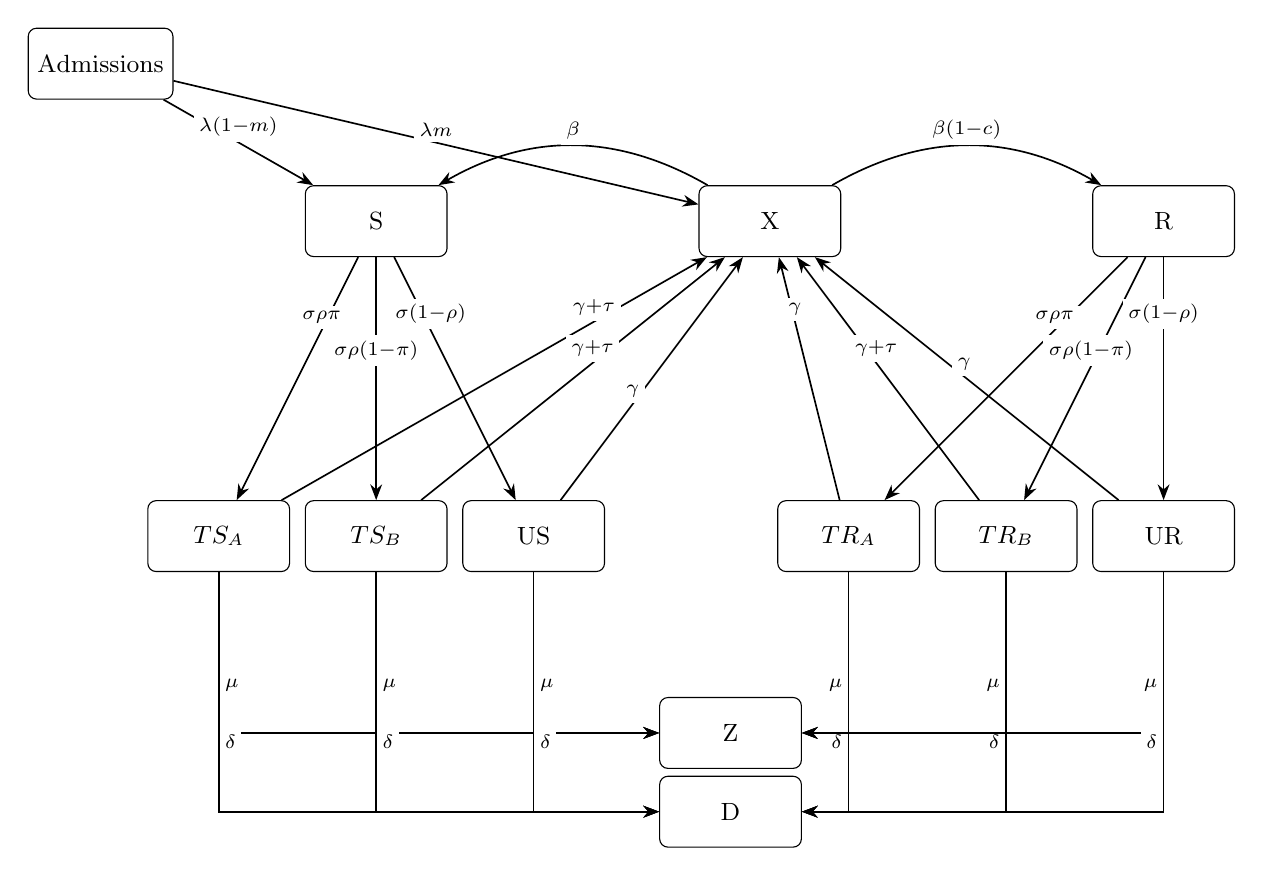
\begin{tikzpicture}[
    >=Stealth,
    box/.style  = {draw, rounded corners=3pt,
                   minimum width=18mm, minimum height=9mm,
                   align=center, font=\small},
    trans/.style = {semithick,->},
    lbl/.style   = {font=\scriptsize, midway, inner sep=2pt, fill=white}
  ]

  \coordinate (origin) at (0,0);

  \node[box] (S) at ($(origin)+( 0, 0)$) {S};
  \node[box] (X) at ($(origin)+( 5, 0)$) {X};
  \node[box] (R) at ($(origin)+(10, 0)$) {R};

  \node[box] (TSA) at ($(S)+( -2,-4)$) {$TS_A$};
  \node[box] (TSB) at ($(S)+(  0,-4)$) {$TS_B$};
  \node[box] (US)  at ($(S)+( 2,-4)$) {US};

  \node[box] (TRA)  at ($(R)+( -4,-4)$) {$TR_A$};
  \node[box] (TRB) at ($(R)+(  -2,-4)$) {$TR_B$};
  \node[box] (UR)  at ($(R)+( 0,-4)$) {UR};

  \node[box] (ADM) at ($(S)+(-3.5, 2)$) {Admissions};

  \node[box] (Z)  at ($(X)+( -0.5,-6.5)$) {Z};
  \node[box] (D)  at ($(X)+(  -0.5,-7.5)$) {D};

  \draw[trans] (ADM) -- (S) node[lbl,above] {$\lambda(1{-}m)$};
  \draw[trans] (ADM) -- (X) node[lbl,above]{$\lambda m$};

  \draw[trans] (S) -- (TSA) node[lbl,pos=0.3,above] {$\sigma\rho\pi$};
  \draw[trans] (S) -- (TSB) node[lbl,pos=0.45,above] {$\sigma\rho(1{-}\pi)$};
  \draw[trans] (S) -- (US)  node[lbl,pos=0.3,above] {$\sigma(1{-}\rho)$};

  \draw[trans] (R) -- (TRA) node[lbl,pos=0.3,above] {$\sigma\rho\pi$};
  \draw[trans] (R) -- (TRB) node[lbl,pos=0.45,above] {$\sigma\rho(1{-}\pi)$};
  \draw[trans] (R) -- (UR)  node[lbl,pos=0.3,above] {$\sigma(1{-}\rho)$};

  \draw[trans] (TSA) -- ($(TSA)!0.55!(X)$) node[lbl,pos=1.3,above] {$\gamma{+}\tau$} -- (X);
  \draw[trans] (TSB) -- ($(TSB)!0.55!(X)$) node[lbl,pos=1,above] {$\gamma{+}\tau$} -- (X);
  \draw[trans] (US)  -- ($(US)!0.55!(X)$)  node[lbl,pos=0.7,above] {$\gamma$} -- (X);

  \draw[trans] (TRA) -- ($(TRA)!0.55!(X)$) node[lbl,pos=1.3,above] {$\gamma$} -- (X);
  \draw[trans] (TRB) -- ($(TRB)!0.55!(X)$) node[lbl,pos=1,above] {$\gamma{+}\tau$} -- (X);
  \draw[trans] (UR)  -- ($(UR)!0.55!(X)$)  node[lbl,pos=0.9,above] {$\gamma$} -- (X);

  \draw[trans] (X) to[out=30,in=150,looseness=1] node[lbl,above] {$\beta(1{-}c)$} (R);
  \draw[trans] (X) to[out=150,in=30,looseness=1] node[lbl,above] {$\beta$} (S);

  \foreach \n in {TSA,TSB,US} {
  \draw[trans] (\n.south) -- ++(0,-6mm) node[lbl,pos=2.4, right]{$\mu$} |- (Z.west);
  \draw[trans] (\n.south) -- ++(0,-6mm) node[lbl, pos=3.6, right]{$\delta$} |- (D.west);
  }

  \foreach \n in {TRA,TRB,UR} {
  \draw[trans] (\n.south) -- ++(0,-6mm) node[lbl,pos=2.4, left]{$\mu$} |- (Z.east);
  \draw[trans] (\n.south) -- ++(0,-6mm) node[lbl, pos=3.6, left]{$\delta$} |- (D.east);
  }

  \end{tikzpicture}
  }%
  \caption*{\textbf{eFigure 1.} State-transition diagram for the hospital transmission ABM. Agents transition between uninfected ($X$), colonized ($S$, $R$), symptomatic/treated ($TS_A$, $TS_B$, $TR_A$, $TR_B$), symptomatic/untreated ($US$, $UR$), discharged ($Z$), and deceased ($D$) states. Drug~A covers only susceptible strains; Drug~B covers both.}
\end{figure}

\end{document}
